
我们刚刚把\trFloerHomology{} $HF_{\star}(H,J)$ 定义为\trComplex{} $CF_{\star}(H,J)$
的\trHomology。本章的目的就是要证明：\trHomology{} $HF_{\star}(H,J)$ 不依赖于所选定的\trRegular{}偶对
$(H,J)\in(\scr{H}\times\scr{J})_{\mathrm{reg}}$（在\cref{sec:results}的意义下）。

为了证明这一点，我们将使用一种方法，它类似于使我们得以在\cref{sec:homology-independence}中
证明\trMorseHomology{}之\trInvariance{}的那个方法。我们将按如下方式进行：设
$(H^{a},J^{a})$ 与 $(H^{b},J^{b})$ 是 $(\scr{H}\times\scr{J})_{\mathrm{reg}}$ 中的两个偶对。
我们考虑一条把 $(H^{a},J^{a})$ 连接到 $(H^{b},J^{b})$ 的\trSmooth\trHomotopy{}
$\varGamma=(H,J)$；更确切地说，
\[
H\colon\RR\times S^{1}\times W\longrightarrow\RR
\qquad\text{与}\qquad
J\colon\RR\longrightarrow\operatorname{End}(TW)
\]
其中对每个 $s$ 都有 $J(s)\in\scr{J}$，并且
\[
\left\{\begin{array}{ll}
H(s,\cdot,\cdot)=H^{a} & \text{若 } s\le-R\\
H(s,\cdot,\cdot)=H^{b} & \text{若 } s\ge R
\end{array}\right.
\qquad\text{与}\qquad
\left\{\begin{array}{ll}
J(s)=J^{a} & \text{若 } s\le-R\\
J(s)=J^{b} & \text{若 } s\ge R\text{。}
\end{array}\right.
\]
这里的 $R$ 是一个常数（对于所有的\trHomotopy{}而言，它未必都取同一个值）。这样的\trHomotopy{}
的存在性源于 $\scr{J}$ 是\trContractible{}的这一事实（\cref{thm:calibrated-section-existence}）。

证明分两步进行：
\begin{enumerate}[label=(\arabic*)]
\item 从一条\trHomotopy{} $\varGamma$ 出发，我们（在 §11.1 与 §11.2 中）定义\trComplex{}的一个\trMorphism
\[
\Phi^{\varGamma}\colon CF_{\star}(H^{a},J^{a})\longrightarrow CF_{\star}(H^{b},J^{b})
\]
并且我们验证：对于把 $(H^{a},J^{a})$ 连接到其自身的\trStationary\trHomotopy{} $\varGamma$，
这个\trMorphism{} $\Phi^{\varGamma}$ 是恒等映射（\cref{thm:phi-gamma-stationary-id}）。
\item 若 $(H^{a},J^{a})$、$(H^{b},J^{b})$ 与 $(H^{c},J^{c})$ 是
$(\scr{H}\times\scr{J})_{\mathrm{reg}}$ 中的偶对，而 $\varGamma$、$\varGamma'$ 与 $\varGamma''$
分别是把 $(H^{a},J^{a})$ 连接到 $(H^{c},J^{c})$、把 $(H^{a},J^{a})$ 连接到 $(H^{b},J^{b})$
以及把 $(H^{b},J^{b})$ 连接到 $(H^{c},J^{c})$ 的\trHomotopy，那么我们将证明：诸\trMorphism
\[
\Phi^{\varGamma''}\circ\Phi^{\varGamma'}
\qquad\text{与}\qquad
\Phi^{\varGamma}\colon CF_{\star}(H^{a},J^{a})\longrightarrow CF_{\star}(H^{c},J^{c})
\]
是相互\trHomotopic{}的，从而特别地在\trHomology{}层面上诱导出同一个\trMorphism。
这第二步本身又分成两个子步骤：
\begin{enumerate}[label=(\alph*)]
\item 我们首先证明：两条\trHomotopy{} $\varGamma_{1}$ 与 $\varGamma_{2}$ 定义出\trHomotopic
{}\trMorphism{} $\Phi^{\varGamma_{1}}$ 与 $\Phi^{\varGamma_{2}}$（命题~11.2.8，在 §11.3 与
§11.4 中证明）。
\item 随后我们证明：存在一条\trHomotopy{} $\varGamma$，使得\trComplex{}的诸\trMorphism{}
$\Phi^{\varGamma''}\circ\Phi^{\varGamma'}$ 与 $\Phi^{\varGamma}$ 相重合（命题~11.2.9，在 §11.5 中证明）。
\end{enumerate}
\end{enumerate}

如同\cref{sec:homology-independence}中那样，我们随后通过考虑 $(H^{a},J^{a})=(H^{c},J^{c})$
且 $\varGamma=\mathrm{Id}$ 的特殊情形，来推出\trFloerHomology{}的\trInvariance。显然，此时
$\Phi^{\varGamma'}$ 与 $\Phi^{\varGamma''}$ 在\trHomology{}层面上诱导出的\trIsomorphism{}互为逆映射。

\section{\trMorphism{} \texorpdfstring{$\Phi^{\varGamma}$}{Phi(Gamma)}}
\label{sec:morphism-phi-gamma}

\subsection{带参数的\trFloerEquation}
\label{subsec:floer-equation-parameters}

设 $\varGamma(s)=(H_{s,t},J_{s})$，并考虑方程
\[
\frac{\partial u}{\partial s}+J_{s}(u)\frac{\partial u}{\partial t}
+\operatorname{grad}_{u}H_{s,t}=0
\]
它也可以写成
\[
\frac{\partial u}{\partial s}+J_{s}(u)\Bigl(\frac{\partial u}{\partial t}
-X_{s,t}(u)\Bigr)=0\text{，}
\]
其中 $X_{s,t}$ 是 $dH_{s,t}$ 的\textbf{\trSymplecticDual}（symplectic dual）。如果 $u$ 是一个解，那么我们就把它的\trEnergy{}定义为
\[
E(u)=\int_{-\infty}^{+\infty}\int_{S^{1}}
\Bigl\|\frac{\partial u}{\partial s}\Bigr\|^{2}\,dt\,ds\text{。}
\]
我们所用的范数是与\trMetric{} $\omega(\cdot\,,J_{s})$ 相联系的那一个——因此它依赖于 $s$。

考虑空间
\[
\scr{M}^{\varGamma}=\bigl\{u\colon\RR\times S^{1}\to W\ \bigm|\ u\text{ 是一个\trContractible{}的解，并且 }E(u)<+\infty\bigr\}\text{。}
\]
我们回想一下：\trHomotopy{} $\varGamma$ 已被定义为在 $|s|\ge R$ 时是\trStationary{}的。这使得我们能够给出一些证明，它们或多或少地类似于第~6~章的那些陈述的下述带参数的版本。

我们首先给出\cref{thm:trajectories-tend-critical-points}的一个带参数的版本。

\begin{theorem}\label{thm:gamma-limits-critical-points}
设 $X^{a}$ 与 $X^{b}$ 分别是\trForm{} $dH^{a}$ 与 $dH^{b}$ 的\textbf{\trSymplecticDual}（symplectic dual）。假定 $X^{a}$ 与
$X^{b}$ 的所有 1-\trPeriodic\trTrajectory{}都是\trNondegenerate{}的。那么对每个
$u\in\scr{M}^{\varGamma}$，存在 $\scr{A}_{H^{a}}$ 的一个\trCriticalPoint{} $x$ 与
$\scr{A}_{H^{b}}$ 的一个\trCriticalPoint{} $y$，使得
\[
\lim_{s\to-\infty}u(s,\cdot)=x(\cdot)
\qquad\text{与}\qquad
\lim_{s\to+\infty}u(s,\cdot)=y(\cdot)\text{。}
\]
\end{theorem}

令
\[
\scr{M}^{\varGamma}(x,y)=\Bigl\{u\in\scr{M}^{\varGamma}\ \Bigm|\
\lim_{s\to-\infty}u(s)=x\ \text{且}\ \lim_{s\to+\infty}u(s)=y\Bigr\}\text{。}
\]
于是，$\scr{M}^{\varGamma}(x,y)$ 的一个元素就是一条\trTrajectory，它在 $s\le-R$ 时沿着
$\scr{A}_{H^{a}}$ 的\trGradient{}的一条\trTrajectory{}从 $x$ 出发，而在 $s\ge R$ 时沿着
$\scr{A}_{H^{b}}$ 的\trGradient{}的一条\trTrajectory{}到达 $y$。从而，每个\trEnergy{}有限的解
都分别把 $\scr{A}_{H^{a}}$ 与 $\scr{A}_{H^{b}}$ 的两个\trCriticalPoint{}连接起来。

当 $s\le-R$ 或 $s\ge R$ 时，我们的方程分别与 $(H^{a},J^{a})$ 或 $(H^{b},J^{b})$ 的
（不带参数的）\trFloerEquation{}相重合。从而，\cref{thm:gamma-limits-critical-points}
可以按一种与\cref{thm:trajectories-tend-critical-points}类似的方式来证明：我们先照搬
\cref{thm:action-tends-critical-values}的证明，以证明对每个 $u\in\scr{M}^{\varGamma}$，
存在两个\trCriticalPoint{} $x\in\operatorname{Crit}(\scr{A}_{H^{a}})$ 与
$y\in\operatorname{Crit}(\scr{A}_{H^{b}})$，使得
\[
\lim_{s\to-\infty}\scr{A}_{H^{a}}(u(s))=\scr{A}_{H^{a}}(x)
\qquad\text{与}\qquad
\lim_{s\to+\infty}\scr{A}_{H^{b}}(u(s))=\scr{A}_{H^{b}}(y)\text{。}
\]

随后我们来证明下面这个结果。

\begin{proposition}\label{thm:energy-upper-bound}
存在一个常数 $k$，使得对每个 $u\in\scr{M}^{\varGamma}$——只要它对\trCriticalPoint{}
$x\in\operatorname{Crit}(\scr{A}_{H^{a}})$ 与 $y\in\operatorname{Crit}(\scr{A}_{H^{b}})$
满足上面的那些条件——我们就有
\[
E(u)\le\scr{A}_{H^{a}}(x)-\scr{A}_{H^{b}}(y)+k\text{。}
\]
\end{proposition}

\begin{proof}
我们有
\[
\begin{aligned}
E(u)&=\int_{\RR\times S^{1}}\Bigl\|\frac{\partial u}{\partial s}\Bigr\|^{2}\,ds\,dt\\
&=\int_{\RR\times S^{1}}\Bigl\langle\frac{\partial u}{\partial s},\,\frac{\partial u}{\partial s}\Bigr\rangle ds\,dt\\
&=\int_{\RR\times S^{1}}\omega\Bigl(\frac{\partial u}{\partial s},\,J_{s}\frac{\partial u}{\partial s}\Bigr)ds\,dt\\
&=\int_{\RR\times S^{1}}\omega\Bigl(\frac{\partial u}{\partial s},\,\frac{\partial u}{\partial t}-X_{s,t}\Bigr)ds\,dt\\
&=\int_{\RR\times S^{1}}u^{\star}\omega-dH_{s,t}\Bigl(\frac{\partial u}{\partial s}\Bigr)ds\,dt\text{。}
\end{aligned}
\]
由于 $x$ 的\trContractible{}性，现在我们可以选取 $u$ 的一个扩张\footnote{译注：原书此页链式等式第四、五行中的两个下标均印作 $X_{t,s}$ 与 $dH_{t,s}$；按本节开头对 $\varGamma(s)=(H_{s,t},J_{s})$ 与 $X_{s,t}$ 的记号约定（本证明第二段随后亦用 $dH_{s,t}$），疑应为 $X_{s,t}$ 与 $dH_{s,t}$。此处径改。——译者注}，也就是说，一个映射
\[
\widetilde{u}\colon\RR\times D^{2}\longrightarrow W
\qquad\text{满足 }\ \widetilde{u}|_{\partial D^{2}}=u\text{。}
\]
我们利用这个扩张来确定 $u$ 的\trEnergy：
\[
\begin{aligned}
E(u)&=\lim_{\sigma\to+\infty}\int_{[-\sigma,\sigma]\times S^{1}}
u^{\star}\omega-dH_{s,t}\Bigl(\frac{\partial u}{\partial s}\Bigr)ds\,dt\\
&=\lim_{\sigma\to+\infty}\Biggl(\int_{[-\sigma,\sigma]\times S^{1}}u^{\star}\omega
+\int_{[-\sigma,\sigma]\times S^{1}}-\frac{\partial}{\partial s}H_{s,t}(u)
+\frac{\partial H}{\partial s}(u)\,ds\,dt\Biggr)\\
&=\lim_{\sigma\to+\infty}\Biggl(\int_{D^{2}}\widetilde{u}_{\sigma}^{\star}\omega
-\int_{D^{2}}\widetilde{u}_{-\sigma}^{\star}\omega
-\int_{S^{1}}H^{b}_{t}(u_{\sigma})\,dt+\int_{S^{1}}H^{a}_{t}(u_{-\sigma})\,dt\\
&\qquad\qquad+\int_{[-R,R]\times S^{1}}\frac{\partial H}{\partial s}(u)\,ds\,dt\Biggr)\text{，}
\end{aligned}
\]
其中
\[
u_{\pm\sigma}(t)=u(\pm\sigma,t)\quad\text{对于 } t\in S^{1}
\qquad\text{与}\qquad
\widetilde{u}_{\pm\sigma}(z)=\widetilde{u}(\pm\sigma,z)\quad\text{对于 } z\in D^{2}\text{。}
\]
我们用到了\trHomotopy{} $H_{s,t}$ 在 $|s|\ge R$ 时是\trStationary{}的这一事实。由此（利用诸假设）便得到
\[
\begin{aligned}
E(u)&=\lim_{\sigma\to+\infty}\bigl(\scr{A}_{H^{a}}(u_{-\sigma})
-\scr{A}_{H^{b}}(u_{\sigma})\bigr)
+\int_{[-R,R]\times S^{1}}\frac{\partial H}{\partial s}(u)\,ds\,dt\\
&=\scr{A}_{H^{a}}(x)-\scr{A}_{H^{b}}(y)
+\int_{[-R,R]\times S^{1}}\frac{\partial H}{\partial s}(u)\,ds\,dt\text{，}
\end{aligned}
\]
我们令
\[
k=\sup_{\substack{s\in[-R,R]\\ t\in S^{1}\\ z\in W}}\frac{\partial H}{\partial s}(s,t,z)
\]
来得到
\[
E(u)\le\scr{A}_{H^{a}}(x)-\scr{A}_{H^{b}}(y)+k
\]
并结束这条命题的证明。\footnote{译注：这个 $k$ 漏掉了积分区间的长度。上一页已经得到 $E(u)=\scr{A}_{H^{a}}(x)-\scr{A}_{H^{b}}(y)+\int_{[-R,R]\times S^{1}}\frac{\partial H}{\partial s}(u)\,ds\,dt$，故误差项 $\int_{[-R,R]\times S^{1}}\frac{\partial H}{\partial s}(u)\,ds\,dt$ 以 $2R\cdot\max\bigl(0,\ \sup_{[-R,R]\times S^{1}\times W}\frac{\partial H}{\partial s}\bigr)$ 为上界（区间 $[-R,R]$ 的长度是 $2R$），即应取 $k=2R\max\bigl(0,\ \sup\frac{\partial H}{\partial s}\bigr)$。按字面取 $k=\sup\frac{\partial H}{\partial s}$ 时不等式可以失效：例如取 $H_{s,t}=H_{0}+\epsilon s$（$\epsilon>0$，$H_{0}$ 有\trCriticalPoint{} $x_{0}$），则 $u\equiv x_{0}$ 是一个常值解，$E(u)=0$，而由上一页的等式 $\scr{A}_{H^{a}}(x_{0})-\scr{A}_{H^{b}}(x_{0})=-2R\epsilon$，且 $\sup\frac{\partial H}{\partial s}=\epsilon$，原书的不等式将读作 $0\le\epsilon-2R\epsilon$，当 $R>\frac{1}{2}$ 时不成立。此处照原书排印。——译者注}
\end{proof}

$\scr{A}_{H^{a}}$ 与 $\scr{A}_{H^{b}}$ 的\trCriticalPoint{}个数的有限性导致了下面的推论
（类似于\cref{thm:uniform-energy-bound}）。

\begin{corollary}\label{thm:uniform-energy-gamma}
存在一个实数 $C>0$，使得对每个 $u\in\scr{M}^{\varGamma}$，都有 $E(u)\le C$。
\end{corollary}

这个结果使我们得以证明一个类似于\cref{thm:gromov-compactness-theorem}的\trCompact{}性质。

\begin{theorem}\label{thm:moduli-gamma-compact}
\trTrajectory{}空间 $\scr{M}^{\varGamma}$ 对于 $\cC^{\infty}_{\mathrm{loc}}(\RR\times S^{1},W)$
\trTopology{}是\trCompact{}的。
\end{theorem}

其证明在一切细节上都类似于\cref{thm:gromov-compactness-theorem}的证明；它依赖于下面的这条命题
（它类似于\cref{thm:uniform-gradient-bound}）。

\begin{proposition}\label{thm:uniform-grad-gamma-bound}
存在一个常数 $A>0$，使得
\[
\forall u\in\scr{M}^{\varGamma},\ \forall(s,t)\in\RR\times S^{1},\quad
\bigl\|\operatorname{grad}_{(s,t)}u\bigr\|\le A\text{。}
\]
\end{proposition}

\noindent\textbf{注记。}这条证明，就如同\cref{thm:uniform-gradient-bound}的证明那样，使用了
\cref{thm:uniform-energy-gamma}（它类似于\cref{thm:uniform-energy-bound}），并且用反证法进行。
如果结论不成立，那么我们就可以推出一个映射 $v\colon\RR^{2}\to W$ 的存在性，使得
\[
\frac{\partial v}{\partial s}+J(s)\frac{\partial v}{\partial t}=0\text{。}
\]
这并不完全是一条如\cref{thm:uniform-gradient-bound}的证明中那样的\trHolomorphic{}曲线，因为
$J$ 依赖于 $s$，但是这个证明可以借助诸\trMetric
\[
g_{s}(\cdot\,,\cdot)=\omega(\cdot\,,J(s)\cdot)
\]
以类似的方式进行。特别地，为了计算 $v(\RR^{2})$ 的面积与 $v(\partial B(0,r_{k}))$ 的长度
（一如\cref{thm:boundary-length-sequence}的证明中那样），我们必须使用由
\[
g_{v(s,t)}(\cdot\,,\cdot)=\omega_{v(s,t)}(\cdot\,,J(s)\cdot)
\]
所定义的\trMetric{} $g$。

利用\cref{thm:moduli-gamma-compact}，我们可以按照与\cref{thm:trajectories-tend-critical-points}
的证明相同的方式结束\cref{thm:gamma-limits-critical-points}的证明。为此，我们需要一个类似于
\cref{thm:subsequence-tends-critical-point}的结果，而后者可以借助下面的\cref{thm:translation-limit-stationary}、
以类似的方式得到证明。

\subsection{\trTransversality}
\label{subsec:transversality-gamma}

我们回到第~8~章的那些结果，并把它们\trAdapted{}到带参数的\trFloerEquation{}上。正如我们将要看到的，
对 $s$ 的依赖性将会简化其中的一些证明：一个更大的源空间将会使\trSurjective{}性更容易证明。
与前面一样，设 $\varGamma=(H,J)$ 是一条把 $(H^{a},J^{a})$ 连接到 $(H^{b},J^{b})$ 的\trHomotopy。
我们引进由（\trPerturbation）函数
\[
h\colon\RR\times S^{1}\times W\longrightarrow\RR
\]
所成的空间 $\cC^{\infty}_{\varepsilon}$，它们具有紧\trSupport{}且满足
$\|h\|_{\varepsilon}<+\infty$。\footnote{译注：按此定义的空间（紧\trSupport{}＋$\|h\|_{\varepsilon}<+\infty$）在范数 $\|\cdot\|_{\varepsilon}$ 下并不完备，而本章的\trTransversality{}论证（对\trImplicitFunctionTheorem{}与\trSard--\trSmale{}定理的应用）需要完备性。病因在于：$\|\cdot\|_{\varepsilon}=\sum_{k\ge0}\varepsilon_{k}\sup|d^{k}h|$（第~8~章的同名范数）只对各阶导数的一致大小加权，完全不控制\trSupport{}的大小——取定一个紧支的 $b$，把它的诸平移 $b(\cdot-j)$ 按幅度随权重衰减的方式加权求和，则部分和都是本空间的元素且构成 $\|\cdot\|_{\varepsilon}$-\trCauchy{}序列，但其极限的\trSupport{}无界，不属于本空间。修补有两条路：或对全体 $h$ 固定一个共同的紧\trSupport（这给出一个完备的闭子空间），或改用按该范数完备的衰减空间（即去掉紧支要求，只保留 $\|h\|_{\varepsilon}<+\infty$——第~8~章的 $\cC^{\infty}_{\varepsilon}$ 正是如此界定的）。两条路都须重写下文的端点论证（$\varGamma(h)$ 在 $\lambda$ 近于 $0$、$1$ 时为\trStationary，靠的正是 $h$ 的紧支性）；若取固定\trSupport，则“对每个 $h\in\cC^{\infty}_{\varepsilon}$”型的全域结论也须加上\trSupport{}方面的限定——例如\cref{thm:z-identically-zero}的结论“则 $Z$ 恒等于零”。\cref{subsec:transversality-gamma-lambda}（原书 p.415）定义 $[0,1]\times\RR\times S^{1}\times W$ 上的同类空间时同病。两处均照原书排印，存疑备案。——译者注}由于 $h$ 具有（关于 $s$ 的）紧\trSupport，\trPerturbation{}后的\trHomotopy
{}在诸\trCriticalPoint{}附近的\trFloer\trTrajectory{}就与未\trPerturbation{}的\trHomotopy{}的那些相同。

现在让我们给出\cref{thm:regular-perturbations}与\cref{thm:moduli-manifold-dimension}的
带参数的版本。

\begin{theorem}\label{thm:transversality-gamma}
存在 $\cC^{\infty}_{\varepsilon}$ 中的一个 $0$ 的邻域，以及此邻域内 $\scr{H}_{\mathrm{reg}}$
的诸\trDense\trOpen{}子集的一个可数交，使得若 $h\in\scr{H}_{\mathrm{reg}}$，则令
$\varGamma(h)=(H+h,J)$，对每个 $x\in\operatorname{Crit}\scr{A}_{H^{a}}$ 与每个
$y\in\operatorname{Crit}\scr{A}_{H^{b}}$，\trTrajectory{}空间 $\scr{M}^{\varGamma(h)}(x,y)$
是一个维数为 $\mu(x)-\mu(y)$ 的\trManifold。此外，对每个 $u\in\scr{M}^{\varGamma(h)}(x,y)$，\trDifferential
\[
(d\scr{F}^{\varGamma(h)})_{u}\colon W^{1,p}(u^{\star}TW)\longrightarrow L^{p}(u^{\star}TW)
\]
是\trSurjective{}的。\footnote{译注：本定理有两处记号疑误。其一，原文印作“此邻域内
$\scr{H}_{\mathrm{reg}}$ 的诸\trDense\trOpen{}子集的一个可数交”；按第~8~章定理~8.1.1 的口径
（彼处 $\scr{H}_{\mathrm{reg}}$ 即诸\trDense\trOpen{}子集之交本身的名字），疑应作“诸%
\trDense\trOpen{}子集的一个可数交 $\scr{H}_{\mathrm{reg}}$”之类。其二，“此外”句中的 $u$ 与%
\trDifferential，原文又印作
$u\in\scr{M}^{\varGamma}(x,y)$ 与 $(d\scr{F}^{\varGamma})_{u}$；按本定理刚定义的
$\varGamma(h)=(H+h,J)$（\trSurjective{}性正是\trPerturbation{}所要保证的），疑应作 $\scr{M}^{\varGamma(h)}(x,y)$ 与
$(d\scr{F}^{\varGamma(h)})_{u}$。前者照原书排印，存疑备案；后者径改。——译者注}
\end{theorem}

出于简单性的考虑，我们在记号中略去了这样一个事实：\trMaslovIndex{} $\mu(x)$ 与 $\mu(y)$
分别是借助 $X^{a}$ 与 $X^{b}$ 的\trFlow{}来计算的。

\cref{thm:transversality-gamma}的证明或多或少地类似于\cref{thm:moduli-manifold-dimension}
的证明。令
\[
\scr{F}^{\varGamma}\colon W^{1,p}(\RR\times S^{1},u^{\star}TW)\longrightarrow
L^{p}(\RR\times S^{1},u^{\star}TW)
\]
由
\[
\scr{F}^{\varGamma}(u)=\frac{\partial u}{\partial s}
+J_{s}\Bigl(\frac{\partial u}{\partial t}-X_{s,t}\Bigr)
\]
所定义。\cref{thm:transversality-gamma}的证明的主要成分是\cref{thm:fgamma-fredholm}，即
\cref{thm:floer-map-fredholm}的类似物。

\begin{theorem}\label{thm:fgamma-fredholm}
对每个 $u\in\scr{M}^{\varGamma}(x,y)$，$\scr{F}^{\varGamma}$ 的\trLinearization{}都是一个%
\trIndex{}为 $\mu(x)-\mu(y)$ 的\trFredholmOperator。
\end{theorem}

其证明与\cref{thm:floer-map-fredholm}的证明相同，因为由于 $\varGamma$ 在 $|s|\ge R$ 时是%
\trStationary{}的，\trLinearization{}算子 $(d\scr{F}^{\varGamma})_{u}$ 在沿着 $u$ 的一个\trUnitary{}基下写出时，
与\trLinearization{}算子 $(d\scr{F})_{u}$ 具有同样的形状：
\[
(d\scr{F}^{\varGamma})_{u}(Y)=\bar{\partial}Y+SY\text{，}
\]
其中 $S(s,t)$ 是一个当 $s\to\pm\infty$ 时趋于一个\trSymmetricMatrix{}的矩阵。

仿照第~8~章的先例——更确切地说，仿照其中概述的那个证明纲要——\cref{thm:fgamma-fredholm}
将用来证明\cref{thm:z-banach-manifold}的带参数的版本，而后者借助\trImplicitFunctionTheorem{}是
下面的\cref{thm:transversality-property}的类似物的一个直接推论。

\begin{proposition}\label{thm:phi-surjective-right-inverse}
设 $\varGamma=(H_{0},J_{0})$ 是 $(H^{a},J^{a})$ 与 $(H^{b},J^{b})$ 之间的一条\trHomotopy。如果
$u\in\scr{M}^{\varGamma}(x,y)$，那么映射
\[
\begin{array}{c}
\Phi\colon W^{1,p}(u^{\star}TW)\times\cC^{\infty}_{\varepsilon}(H_{0})
\longrightarrow L^{p}(u^{\star}TW)\\[4pt]
(Y,h)\longmapsto(d\scr{F}^{\varGamma})_{u}(Y)+\operatorname{grad}_{u}h
\end{array}
\]
\footnote{译注：原书此映射的源空间与目标空间印作 $W^{1,p}(u^{\star}W)$ 与
$L^{p}(u^{\star}W)$；按 $Y$ 为沿 $u$ 的\trVectorField{}（下面的\cref{thm:z-identically-zero}
亦用 $L^{q}(u^{\star}TW)$），疑应为 $u^{\star}TW$。此处径改。——译者注}
是\trSurjective{}的，并且具有一个右逆。
\end{proposition}

\begin{proof}
$\cC^{\infty}_{\varepsilon}(H_{0})$ 中的那些\trHamiltonian{}量对 $s$ 的依赖性，与
\cref{thm:transversality-property}的证明相比，大大地简化了\trSurjective{}性的证明：源空间更大了。
我们不再需要\trRegularity{}（即\cref{thm:critical-points-discrete}），也不再需要解释这个概念的
\cref{sec:somewhere-injective}。以下是细节。

如同\cref{sec:transversality}中那样，我们先以类似于\cref{thm:z-pairing-vanish}的方式来证明：
如果 $\Phi$ 不是\trSurjective{}的，那么就存在一个非零的\trVectorField{}
$Z\in L^{q}(u^{\star}TW)$（$q$ 满足 $1/p+1/q=1$），它是 $\cC^{\infty}$ 类的，并且使得对每个
$h\in\cC^{\infty}_{\varepsilon}(H_{0})$ 与每个 $Y\in W^{1,p}(u^{\star}TW)$，都有
\[
\bigl\langle Z,\,(d\scr{F}^{\varGamma})_{u}(Y)\bigr\rangle=0
\qquad\text{与}\qquad
\bigl\langle Z,\,\operatorname{grad}_{u}(h)\bigr\rangle=0\text{。}
\]

接下来，我们把\cref{thm:z-lambda-grad}换成下面的更强的结果。

\begin{lemma}\label{thm:z-identically-zero}
如果 $Z\in L^{q}(u^{\star}TW)\cap\cC^{\infty}(\RR\times S^{1};TW)$ 满足
\[
\bigl\langle Z,\,\operatorname{grad}_{u}h\bigr\rangle=0
\qquad\text{对每个 } h\in\cC^{\infty}_{\varepsilon}(H_{0})\text{，}
\]
那么 $Z$ 恒等于零。
\end{lemma}

由于这条引理与上文相矛盾，我们便推出 $\Phi$ 是\trSurjective{}的。它具有一个右逆，这仍然是依据
\cref{thm:continuous-right-inverse}。\cref{thm:phi-surjective-right-inverse}得证。
\end{proof}

\begin{proof}[\cref{thm:z-identically-zero}的证明]
作为引理之假设的那个关系式可以改写为
\[
\int_{\RR\times S^{1}}dh(Z)\,ds\,dt=0
\qquad\text{对每个 } h\in\cC^{\infty}_{\varepsilon}(H_{0})\text{。}
\]
考虑映射
\[
\begin{array}{c}
\widetilde{u}\colon\RR\times S^{1}\longrightarrow W\times\RR\times S^{1}\\[2pt]
(s,t)\longmapsto(u(s,t),s,t)\text{。}
\end{array}
\]
容易证明：$\widetilde{u}$ 是一个\trEmbedding。我们把 $Z$ 视为 $W\times\RR\times S^{1}$ 上沿着
$\widetilde{u}$ 的一个\trVectorField，它在方向 $\partial/\partial t\in TS^{1}$ 与
$\partial/\partial s\in T\RR$ 上没有任何分量。特别地，在 $Z$ 非零的那些点处，$Z$ 不在切于
$\widetilde{u}$ 的平面之中。

为了导出矛盾，我们假定这样的点 $(s_{0},t_{0})\in\RR\times S^{1}$ 确实存在。我们完全按照
\cref{thm:z-lambda-grad}的证明来进行：我们考虑 $\RR\times S^{1}$ 中 $(s_{0},t_{0})$ 的一个小邻域
$C_{\delta}$，使得 $Z(s,t)$ 在这个邻域内的诸 $(s,t)$ 处非零（从而\trTransverse{}于
$\widetilde{u}$）。我们取
一个\trSupport{}在这个邻域内的函数
\[
\beta\colon\RR\times S^{1}\longrightarrow\RR
\]
并定义一个\trSupport{}在 $\widetilde{u}(C_{\delta})$ 的一个\trTubularNeighborhood{} $B$ 内的
$h\in\cC^{\infty}_{\varepsilon}(H_{0})$，使得：若 $\gamma_{(s,t)}(\sigma)$ 是 $Z$ 的那条当
$\sigma=0$ 时经过 $\widetilde{u}(s,t)$ 的\trIntegralCurve，则我们有
\[
h_{s,t}\bigl(\gamma_{(s,t)}(\sigma)\bigr)=\beta(s,t)\cdot\sigma
\qquad\text{对于 } |\sigma|\le\eta
\]
（其中 $\eta>0$ 充分小）。由于 $Z$ \trTransverse{}于 $\widetilde{u}(C_{\delta})$，函数 $h$ 是%
\trWellDefined{}的。我们还假定
\[
B\cap\operatorname{Im}(\widetilde{u})=\widetilde{u}(C_{\delta})\text{，}
\]
这特别地意味着
\[
\operatorname{Supp}(h)\cap\operatorname{Im}(\widetilde{u})
=\widetilde{u}(C_{\delta})
\]
（\cref{fig:tubular-neighborhood-b}）。\footnote{译注：本处与本章下文另有三处小疑误，合并立一枚归组注。其一（原书 p.390，即本处）：由 $B\cap\operatorname{Im}(\widetilde{u})=\widetilde{u}(C_{\delta})$ 与 $\operatorname{Supp}(h)\subseteq B$ 只能得出 $\operatorname{Supp}(h)\cap\operatorname{Im}(\widetilde{u})\subseteq\widetilde{u}(C_{\delta})$——反方向的包含须另验 $\widetilde{u}(C_{\delta})\subseteq\operatorname{Supp}(h)$，而 $\beta$（从而 $h$）本可取得更小，等号无据。其二（原书 p.395）：\cref{thm:broken-limit-gamma}的证明给出的两条破碎链 $(v^{0},v^{1},\dotsc,v^{\ell})$ 与 $(u^{0},u^{1},\dotsc,u^{k})$ 各多写一项——按 $v^{j}\in\scr{M}_{(H^{b},J^{b})}(y_{j},y_{j+1})$、$u^{i}\in\scr{M}_{(H^{a},J^{a})}(x_{i},x_{i+1})$ 以及 $y_{\ell}=y$、$x_{k}=x'$，末端的取值 $j=\ell$、$i=k$ 将用到无定义的 $y_{\ell+1}$ 与 $x_{k+1}$，应为 $0\le j\le\ell-1$ 与 $0\le i\le k-1$（对照\cref{thm:maslov-index-lower-bound}证明中的求和范围）。其三（原书 p.409，§11.2）：选取 $A$、$B$ 时的条件 $[\sigma_{n},\sigma'_{n}]\subset[A,B]$ 是反序的空区间（该证明前文已有 $\sigma'_{n}\le\sigma_{n}$），应为 $[\sigma'_{n},\sigma_{n}]$，彼处径改。其四（原书 p.411，§11.2 末）：$\ell_{n}(s+\rho_{n})=\exp_{w_{\rho_{n}}(s)}\bigl(i_{\rho_{n}}\bigl(\gamma_{n}(h_{n}(s))\bigr)\bigr)$ 中 $\gamma_{n}$ 的自变元印作 $h_{n}(s)$——$\gamma_{n}$ 接收的是整条\trSection{} $h_{n}\in W^{1,p}\bigl(\RR\times S^{1};\RR^{2n}\bigr)$（紧随其后的公式即以 $h$ 为变量），疑应作 $\gamma_{n}(h_{n})$。四处均照原书排印，其三径改。——译者注}

\begin{figure}[htbp]
\centering
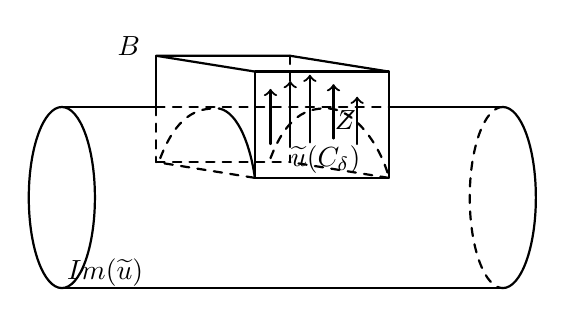
\begin{tikzpicture}[line cap=round,line join=round,x=1cm,y=1cm]
\draw[thick] (-3.0,0) ellipse (0.42 and 1.15);
\draw[thick] (-3.0,1.15) -- (-1.8,1.15);
\draw[dashed,thick] (-1.8,1.15) -- (1.15,1.15);
\draw[thick] (1.15,1.15) -- (2.6,1.15);
\draw[thick] (-3.0,-1.15) -- (2.6,-1.15);
\draw[dashed,thick] (2.6,1.15) arc[start angle=90, end angle=270, x radius=0.42, y radius=1.15];
\draw[thick] (2.6,1.15) arc[start angle=90, end angle=-90, x radius=0.42, y radius=1.15];
\node at (-2.45,-0.95) {$\operatorname{Im}(\widetilde{u})$};
\draw[thick] (-0.55,0.25) rectangle (1.15,1.60);
\draw[thick] (-0.55,1.60) -- (-1.80,1.80) -- (-0.10,1.80) -- (1.15,1.60);
\draw[thick] (-1.80,1.80) -- (-1.80,1.15);
\draw[dashed,thick] (-1.80,1.15) -- (-1.80,0.45);
\draw[dashed,thick] (-0.10,1.80) -- (-0.10,0.45);
\draw[dashed,thick] (-0.55,0.25) -- (-1.80,0.45);
\draw[dashed,thick] (1.15,0.25) -- (-0.10,0.45);
\draw[dashed,thick] (-1.80,0.45) -- (-0.10,0.45);
\node at (-2.15,1.92) {$B$};
\draw[dashed,thick] (-1.75,0.50) .. controls (-1.55,1.02) and (-1.30,1.15) .. (-1.00,1.13);
\draw[thick] (-1.00,1.13) .. controls (-0.75,1.08) and (-0.60,0.62) .. (-0.55,0.26);
\draw[dashed,thick] (-0.35,0.50) .. controls (-0.15,1.02) and (0.10,1.15) .. (0.40,1.13)
  .. controls (0.70,1.11) and (1.02,0.72) .. (1.15,0.27);
\node at (0.35,0.48) {$\widetilde{u}(C_{\delta})$};
\draw[thick,->] (-0.35,0.68) -- (-0.35,1.38);
\draw[thick,->] (-0.10,0.75) -- (-0.10,1.48);
\draw[thick,->] (0.15,0.70) -- (0.15,1.56);
\draw[thick,->] (0.45,0.75) -- (0.45,1.44);
\draw[thick,->] (0.75,0.68) -- (0.75,1.28);
\node at (0.60,0.98) {$Z$};
\end{tikzpicture}
\caption{}
\label{fig:tubular-neighborhood-b}
\end{figure}

于是我们便得到
\[
\begin{aligned}
\int_{\RR\times S^{1}}dh(Z(s,t))\,ds\,dt
&=\int_{C_{\delta}}dh_{s,t}(Z(s,t))\,ds\,dt\\
&=\int_{C_{\delta}}dh_{s,t}\Bigl(\frac{\partial\gamma_{s,t}(\sigma)}{\partial\sigma}
\Bigr|_{\sigma=0}\Bigr)ds\,dt\\
&=\int_{C_{\delta}}\frac{\partial}{\partial\sigma}
\Bigr|_{\sigma=0}h_{s,t}\bigl(\gamma_{(s,t)}(\sigma)\bigr)ds\,dt\\
&=\int_{C_{\delta}}\beta(s,t)\,ds\,dt\text{。}
\end{aligned}
\]
只需这样来选取 $\beta$，使得这个积分不为零，便可导出矛盾，这就证明了：对每个
$(s,t)\in\RR\times S^{1}$ 都有 $Z(s,t)=0$。至此引理得证。
\end{proof}

\cref{thm:transversality-gamma}的证明的结尾部分类似于\cref{thm:regular-perturbations}与
\cref{thm:moduli-manifold-dimension}的证明的结尾部分。

我们将把满足\cref{thm:transversality-gamma}之结论的一条\trHomotopy{}称作
\emph{\trRegular\trHomotopy}。

\noindent\textbf{注记。}由于\trPerturbation{} $h$ 具有紧\trSupport，\trHomotopy{} $\varGamma(h)$
连接 $(H^{a},J^{a})$ 与 $(H^{b},J^{b})$，并且在 $|s|\ge R$ 时是\trStationary{}的
（$R$ 充分大）。

\subsection{\trCompact{}性}
\label{subsec:compactness-gamma}

设 $\varGamma$ 是一条把 $(H^{a},J^{a})$ 连接到 $(H^{b},J^{b})$ 的\trRegular\trHomotopy。我们所
惦记的那个\trMorphism
\[
\Phi^{\varGamma}\colon CF_{\star}(H^{a},J^{a})\longrightarrow CF_{\star}(H^{b},J^{b})
\]
定义如下。对于 $\scr{A}_{H^{a}}$ 的一个\trIndex{}为 $\mu(x)=k$ 的\trCriticalPoint{} $x$，我们令
\[
\Phi^{\varGamma}_{k}(x)=\sum_{\substack{y\in\operatorname{Crit}\scr{A}_{H^{b}}\\ \mu(y)=k}}
n^{\varGamma}(x,y)\,y\text{，}
\]
其中 $n^{\varGamma}(x,y)$ 表示 $\scr{M}^{\varGamma}(x,y)$ 的元素个数（模 $2$）……为了使 $\Phi^{\varGamma}$
是\trWellDefined{}的，我们将需要证明这个数的有限性。我们还需要验证这个 $\Phi^{\varGamma}$ 是\trComplex{}的
一个\trMorphism，也就是说：
\[
\Phi^{\varGamma}\circ\partial_{(H^{a},J^{a})}
=\partial_{(H^{b},J^{b})}\circ\Phi^{\varGamma}\text{。}
\]

为此我们将需要下面这条定理所预告的\trCompact{}性结果，它是\cref{thm:broken-limit-decomposition}
的一个带参数的版本。

\begin{theorem}\label{thm:broken-limit-gamma}
设 $(u_{n})$ 是 $\scr{M}^{\varGamma}(x,y)$ 中诸元素的一个序列。那么存在：
\begin{itemize}
\item $(u_{n})$ 的一个子序列；
\item $\scr{A}_{H^{a}}$ 的\trCriticalPoint{} $x=x_{0},x_{1},\dotsc,x_{k}$；
\item $\scr{A}_{H^{b}}$ 的\trCriticalPoint{} $y_{0},y_{1},\dotsc,y_{\ell}=y$；
\item 使 $0\le i\le k-1$ 的、趋于 $-\infty$ 的实数序列 $(s^{i}_{n})$，以及使
$0\le j\le\ell-1$ 的、趋于 $+\infty$ 的实数序列 $(s^{\prime j}_{n})$；
\item 诸元素 $u^{i}\in\scr{M}_{(H^{a},J^{a})}(x_{i},x_{i+1})$（$0\le i\le k-1$）
与诸元素 $v^{j}\in\scr{M}_{(H^{b},J^{b})}(y_{j},y_{j+1})$（$0\le j\le\ell-1$）；
\item 一个元素 $w\in\scr{M}^{\varGamma}(x_{k},y_{0})$，
\end{itemize}
使得对 $0\le i\le k-1$ 与 $0\le j\le\ell-1$，
\[
\lim_{n\to+\infty}u_{n}\cdot s^{i}_{n}=u^{i}\text{，}\qquad
\lim_{n\to+\infty}u_{n}\cdot s^{\prime j}_{n}=v^{j}\text{，}
\]
并且使得
\[
\lim_{n\to+\infty}u_{n}=w\text{。}
\]
\end{theorem}

这条定理断言：在必要时抽取子序列之后，$\scr{M}^{\varGamma}$ 中的诸\trTrajectory{}序列所具有的极限，
是（至多）一条对应于偶对 $(H^{a},J^{a})$ 的\trBrokenTrajectory、恰好一条 $\scr{M}^{\varGamma}$ 中的%
\trTrajectory{}以及（至多）一条对应于偶对 $(H^{b},J^{b})$ 的\trBrokenTrajectory{}的拼接。

在给出\cref{thm:broken-limit-gamma}的证明之前，我们先陈述它的一个直接推论
（破裂数目的一个上界）。

\begin{figure}[htbp]
\centering
\begin{tikzpicture}[line cap=round,line join=round,x=1cm,y=1cm]
\draw[thick] (-2.35,2.0) ellipse (0.30 and 0.14);
\node at (-2.85,2.08) {$x$};
\draw[thick] (-2.63,1.94) .. controls (-2.52,1.55) and (-2.42,1.10) .. (-2.33,0.70);
\draw[thick] (-2.07,1.95) .. controls (-1.96,1.55) and (-1.86,1.10) .. (-1.77,0.70);
\draw[dashed,thick] (-2.05,0.70) ellipse (0.28 and 0.13);
\draw[thick] (-2.33,0.70) .. controls (-2.15,0.15) and (-1.40,-0.70) .. (-1.03,-1.35);
\draw[thick] (-1.77,0.70) .. controls (-1.55,0.15) and (-0.85,-0.65) .. (-0.47,-1.35);
\draw[dashed,thick] (-0.75,-1.35) ellipse (0.28 and 0.13);
\draw[thick] (-1.03,-1.35) .. controls (-0.97,-1.70) and (-0.80,-2.02) .. (-0.62,-2.20);
\draw[thick] (-0.47,-1.35) .. controls (-0.42,-1.70) and (-0.30,-2.05) .. (-0.02,-2.20);
\draw[thick] (-0.32,-2.20) ellipse (0.30 and 0.14);
\node at (0.42,-2.26) {$y$};
\node at (-1.42,1.50) {$s\le-R$};
\node at (-2.55,-0.30) {$u_{n}$};
\node at (-1.72,-1.80) {$s\ge R$};
\draw[thick] (3.35,2.05) ellipse (0.28 and 0.13);
\node at (2.90,2.12) {$x$};
\draw[thick] (3.09,2.00) .. controls (3.13,1.80) and (3.18,1.60) .. (3.22,1.45);
\draw[thick] (3.61,2.00) .. controls (3.66,1.80) and (3.70,1.60) .. (3.74,1.45);
\draw[thick] (3.28,1.37) .. controls (3.42,1.28) and (3.58,1.17) .. (3.70,1.08);
\draw[thick] (3.68,1.37) .. controls (3.82,1.28) and (3.98,1.17) .. (4.10,1.08);
\draw[dashed,thick] (3.22,1.45) arc[start angle=180, end angle=0, x radius=0.26, y radius=0.12];
\draw[thick] (3.22,1.45) arc[start angle=180, end angle=360, x radius=0.26, y radius=0.12];
\draw[dashed,thick] (3.64,1.00) arc[start angle=180, end angle=0, x radius=0.26, y radius=0.12];
\draw[thick] (3.64,1.00) arc[start angle=180, end angle=360, x radius=0.26, y radius=0.12];
\draw[thick] (3.70,0.92) .. controls (4.10,0.55) and (4.55,0.10) .. (4.87,-0.17);
\draw[thick] (4.10,0.92) .. controls (4.50,0.55) and (4.95,0.10) .. (5.23,-0.17);
\draw[dashed,thick] (4.79,-0.25) arc[start angle=180, end angle=0, x radius=0.26, y radius=0.12];
\draw[thick] (4.79,-0.25) arc[start angle=180, end angle=360, x radius=0.26, y radius=0.12];
\draw[thick] (4.87,-0.33) .. controls (4.75,-0.60) and (4.65,-0.90) .. (4.57,-1.12);
\draw[thick] (5.23,-0.33) .. controls (5.10,-0.60) and (5.00,-0.90) .. (4.93,-1.12);
\draw[dashed,thick] (4.49,-1.20) arc[start angle=180, end angle=0, x radius=0.26, y radius=0.12];
\draw[thick] (4.49,-1.20) arc[start angle=180, end angle=360, x radius=0.26, y radius=0.12];
\draw[thick] (4.57,-1.28) .. controls (4.80,-1.55) and (5.05,-1.80) .. (5.27,-1.95);
\draw[thick] (4.93,-1.28) .. controls (5.15,-1.55) and (5.45,-1.80) .. (5.73,-1.95);
\draw[dashed,thick] (5.18,-2.05) arc[start angle=180, end angle=0, x radius=0.32, y radius=0.14];
\draw[thick] (5.18,-2.05) arc[start angle=180, end angle=360, x radius=0.32, y radius=0.14];
\node at (4.50,1.00) {$x'$};
\node at (4.52,-0.25) {$y'$};
\node at (5.02,-2.12) {$y$};
\node[align=center] at (1.55,1.50) {\small 对应于 $(H^{a},J^{a})$\\ \small 的\trBrokenTrajectory};
\node at (3.45,0.40) {$\lim u_{n}$};
\node[align=center] at (2.75,-1.30) {\small 对应于 $(H^{b},J^{b})$\\ \small 的\trBrokenTrajectory};
\end{tikzpicture}
\caption{}
\label{fig:broken-concatenation-gamma}
\end{figure}

\begin{corollary}\label{thm:maslov-index-lower-bound}
在\cref{thm:broken-limit-gamma}的假设下，
\[
\mu(x)-\mu(y)\ge k+\ell\text{。}
\]
\end{corollary}

\begin{proof}
由\cref{thm:moduli-manifold-dimension}（以及\cref{subsec:space-l-topology}）我们知道：
\[
\left\{\begin{array}{ll}
\scr{M}_{(H^{a},J^{a})}(x_{i},x_{i+1})=\varnothing & \text{若 } \mu(x_{i})-\mu(x_{i+1})<1\\[2pt]
\scr{M}_{(H^{b},J^{b})}(y_{j},y_{j+1})=\varnothing & \text{若 } \mu(y_{j})-\mu(y_{j+1})<1\text{，}
\end{array}\right.
\]
从而，对 $0\le i\le k-1$ 与 $0\le j\le\ell-1$，我们有
\[
\mu(x_{i})-\mu(x_{i+1})\ge1
\qquad\text{与}\qquad
\mu(y_{j})-\mu(y_{j+1})\ge1\text{。}
\]
由\cref{thm:transversality-gamma}，$\scr{M}^{\varGamma}(x_{k},y_{0})\ne\varnothing$ 蕴含
$\mu(x_{k})\ge\mu(y_{0})$。把这些不等式全都加起来，我们就找到了所要的不等式
（回忆一下 $x_{0}=x$ 与 $y_{\ell}=y$）。
\end{proof}

\begin{proof}[\cref{thm:broken-limit-gamma}的证明]
它从一个引理开始。

\begin{lemma}\label{thm:translation-limit-stationary}
设 $(u_{n})$ 是 $\scr{M}^{\varGamma}(x,y)$ 中的一个序列，而 $(s_{n})$ 是一个满足
$\lim s_{n}=+\infty$ 的实数序列。那么存在 $(u_{n})$ 的一个子序列（我们仍把它记作
$(u_{n})$）与一个元素 $v\in\scr{M}_{(H^{b},J^{b})}$，使得 $\lim u_{n}\cdot s_{n}=v$。
同样地，若 $\lim s_{n}=-\infty$，则存在一个 $u\in\scr{M}_{(H^{a},J^{a})}$，使得
（在必要时抽取子序列之后）$\lim u_{n}\cdot s_{n}=u$。
\end{lemma}

\begin{proof}
与前面一样，在记号 $u_{n}=u_{n}(s,t)$ 中我们将省略变量 $t$。当然，只需考虑趋于 $+\infty$
的序列 $(s_{n})$ 的情形就够了。由于 $u_{n}\in\scr{M}^{\varGamma}$，\cref{thm:uniform-grad-gamma-bound}
的结论——即 $\|\operatorname{grad}_{(s,t)}u\|\le A$ 这一事实——对 $u_{n}$ 成立，因而对
$u_{n}\cdot s_{n}$ 也成立，于是 $(u_{n}\cdot s_{n})$ 这个族是\trEquicontinuity{}的，从而由%
\trArzelaAscoliTheorem（必要时参见\cref{sec:appC-arzela-ascoli}），$(u_{n}\cdot s_{n})$ 存在一个子序列，它对于
$\cC^{0}_{\mathrm{loc}}$ \trTopology{}\trConvergence{}到一个连续的极限 $v$。

但是 $v_{n}=u_{n}\cdot s_{n}$ 是\trFloer{}型方程
\[
\frac{\partial v_{n}}{\partial s}
+J_{s+s_{n}}\Bigl(\frac{\partial v_{n}}{\partial t}
-X_{s+s_{n},t}\Bigr)=0
\]
的一个解。\trEllipticRegularity（仍然是\cref{thm:solution-smoothness-regularity}）于是蕴含
$v$ 是 $\cC^{\infty}$ 类的，并且 $(v_{n})$ 在 $\cC^{\infty}_{\mathrm{loc}}$ 中\trConvergence{}到 $v$。

我们还需验证 $v\in\scr{M}_{(H^{b},J^{b})}$。考虑一个闭区间 $[-r,r]\subset\RR$ 与
$\RR\times S^{1}$ 的紧子集 $K=[-r,r]\times S^{1}$。对充分大的 $n$，$s_{n}>R+r$，于是对
$(s,t)\in K$ 与充分大的 $n$，我们有 $s+s_{n}>R$，从而
\[
\frac{\partial v_{n}}{\partial s}
+J^{b}\Bigl(\frac{\partial v_{n}}{\partial t}-X^{b}_{t}(v_{n})\Bigr)=0\text{。}
\]
在这个方程中令 $n$ 趋于无穷，我们的确发现极限 $v$ 落在 $\scr{M}_{(H^{b},J^{b})}$ 之中。
\end{proof}

现在我们可以证明\cref{thm:broken-limit-gamma}了。如同\cref{thm:trajectories-tend-critical-points}
的证明中那样，我们选取 $\varepsilon>0$ 充分小，使得诸开球
\[
B(z,\varepsilon)=\bigl\{\gamma\in\scr{L}W\ \bigm|\ d_{\infty}(z,\gamma)<\varepsilon\bigr\}
\]
对 $z\in\operatorname{Crit}\scr{A}_{H^{a}}$ 两两不交
（对 $z\in\operatorname{Crit}\scr{A}_{H^{b}}$ 同样的性质也成立）。

从现在起，为了简化记号，我们将把必要的子序列抽取略去不写。由于 $\scr{M}^{\varGamma}$ 是%
\trCompact{}的（\cref{thm:moduli-gamma-compact}），我们有 $w=\lim u_{n}\in\scr{M}^{\varGamma}$。
由\cref{thm:gamma-limits-critical-points}，存在 $\scr{A}_{H^{a}}$ 的\trCriticalPoint{} $x'$
与 $\scr{A}_{H^{b}}$ 的\trCriticalPoint{} $y'$，使得 $w\in\scr{M}^{\varGamma}(x',y')$。我们采用
\cref{thm:broken-l-compact}的证明中的论证。存在一个 $s^{\star}\in\RR$，使得对 $s\ge s^{\star}$
都有 $w(s)\in B(y',\varepsilon)$。由于 $w=\lim u_{n}$，我们也有
\[
u_{n}(s^{\star})\in B(y',\varepsilon)
\qquad\text{对充分大的 } n\text{。}
\]
如果 $y'\ne y$（否则就没有什么要证的了），那么这条\trTrajectory{}必定在某个 $s\ge s^{\star}$ 时
穿出球 $B(y',\varepsilon)$。设 $s_{n}$ 是它的首个\trExitPoint：
\[
s_{n}=\sup\bigl\{\,s\ge s^{\star}\ \bigm|\ u_{n}(\sigma)\in B(y',\varepsilon)
\ \text{对于 } \sigma\in[s^{\star},s]\,\bigr\}\text{。}
\]

现在我们将证明序列 $(s_{n})$ 趋于 $+\infty$。我们假定它是\trBounded{}的，从而在必要时抽取一个子序列之后，
它趋于某个 $s_{\bullet}\in\RR$。由于 $(u_{n})$ 向 $w$ 的\trConvergence{}在 $\cC^{\infty}_{\mathrm{loc}}$
中进行，并且由于 $s_{\bullet}\ge s^{\star}$，
\[
\lim_{n\to+\infty}u_{n}(s_{n})=w(s_{\bullet})\in B(y',\varepsilon)\text{。}
\]
然而，按 $s_{n}$ 的定义，我们知道对每个 $n$ 都有 $u_{n}(s_{n})\in\partial B(y',\varepsilon)$，
这与前面的论断相矛盾。

我们这样就证明了 $\lim s_{n}=+\infty$，于是（由\cref{thm:translation-limit-stationary}）
\[
\lim_{n\to+\infty}u_{n}\cdot s_{n}=v^{0}\in\scr{M}_{(H^{b},J^{b})}\text{。}
\]

设 $s<0$。对充分大的 $n$，$s^{\star}<s+s_{n}<s_{n}$，于是按 $s_{n}$ 的定义，
\[
u_{n}(s+s_{n})\in B(y',\varepsilon)
\qquad\text{对充分大的 } n\text{，}
\]
这就蕴含 $v^{0}(s)\in B(y',\varepsilon)$。从而
\[
v^{0}\in\scr{M}_{(H^{b},J^{b})}(y',y_{1})
\qquad\text{对某个 } y_{1}\in\operatorname{Crit}\scr{A}_{H^{b}}\text{。}
\]

证明随后以一种与\cref{thm:broken-l-compact}的证明完全类似的方式继续进行（并结束）：
它导致一个极限，后者是一条\trBrokenTrajectory{} $(v^{0},v^{1},\dotsc,v^{\ell})$，其中
$v^{j}\in\scr{M}_{(H^{b},J^{b})}(y_{j},y_{j+1})$（$y_{0}=y'$ 而 $y_{\ell}=y$）。

我们现在假定 $x'\ne x$。一种类似的推理——利用一个使 $w(s)\in B(x',\varepsilon)$ 对
$s<s_{\star}$ 成立的 $s_{\star}$，然后利用 $u_{n}(s)$ 进入 $B(x',\varepsilon)$ 的最后一个
\textbf{\trEntryPoint}（entry point） $s'_{n}<s_{\star}$——给出了一个趋于 $-\infty$ 的序列 $s'_{n}$，并且对它有
$\lim u_{n}\cdot s'_{n}=u^{\bullet}\in\scr{M}(x_{1},x')$。如同\cref{thm:broken-l-compact}
的证明中那样，这个极限是一条\trBrokenTrajectory{} $(u^{0},u^{1},\dotsc,u^{k})$，其中
$u^{i}\in\scr{M}_{(H^{a},J^{a})}(x_{i},x_{i+1})$（$x_{0}=x$，$x_{k}=x'$）。\cref{thm:broken-limit-gamma}
至此得证。
\end{proof}

\begin{corollary}\label{thm:moduli-gamma-same-index-compact}
若 $\mu(x)=\mu(y)$，那么空间 $\scr{M}^{\varGamma}(x,y)$ 是\trCompact{}的。
\end{corollary}

\begin{proof}
\cref{thm:maslov-index-lower-bound}表明：$\scr{M}^{\varGamma}(x,y)$ 中的一个序列 $(u_{n})$
不可能趋于一条\trBrokenTrajectory。
\end{proof}

于是，映射
\[
\Phi^{\varGamma}_{k}\colon CF_{k}(H^{a},J^{a})\longrightarrow CF_{k}(H^{b},J^{b})
\]
便由公式
\[
\Phi^{\varGamma}_{k}(x)=\sum_{\substack{y\in\operatorname{Crit}\scr{A}_{H^{b}}\\ \mu(y)=k}}
n^{\varGamma}(x,y)\,y
\]
\trWellDefined{}地给出了。我们还将验证下面这个结果。

\begin{proposition}\label{thm:phi-gamma-stationary-id}
若 $(H^{a},J^{a})=(H^{b},J^{b})$ 且 $\varGamma=\mathrm{Id}$，那么对每个 $k$，$\Phi^{\varGamma}_{k}$
都是恒等映射。
\end{proposition}

\begin{proof}
在这个假设下，$\scr{M}^{\varGamma}(x,y)=\scr{M}_{(H^{a},J^{a})}(x,y)$。并且，若此外还有
$\mu(x)=\mu(y)$，那么我们知道（参见\cref{thm:l-dimension-remark}）
\[
\scr{M}_{(H^{a},J^{a})}(x,y)=
\left\{\begin{array}{ll}
\varnothing & \text{若 } x\ne y\\
\{x\} & \text{若 } x=y\text{。}
\end{array}\right.
\]
从而 $\Phi^{\varGamma}_{k}=\mathrm{Id}$。
\end{proof}

为了完成我们为本节定下的那些目标，我们还需要证明 $\Phi^{\varGamma}$ 是\trComplex{}的一个%
\trMorphism，也就是说：
\[
\Phi^{\varGamma}\circ\partial_{(H^{a},J^{a})}
=\partial_{(H^{b},J^{b})}\circ\Phi^{\varGamma}\text{。}
\]

我们必须证明：若 $x\in\operatorname{Crit}\scr{A}_{H^{a}}$，那么对每个使 $\mu(x)-\mu(z)=1$ 的
$z\in\operatorname{Crit}\scr{A}_{H^{b}}$，下面的等式成立（模 $2$）：
\[
\sum_{\substack{y'\in\operatorname{Crit}\scr{A}_{H^{a}}\\ \mu(x)-\mu(y')=1}}
n^{a}(x,y')\,n^{\varGamma}(y',z)
=
\sum_{\substack{y\in\operatorname{Crit}\scr{A}_{H^{b}}\\ \mu(x)=\mu(y)}}
n^{\varGamma}(x,y)\,n^{b}(y,z)\text{，}
\]
（不用说，$n^{a}$ 与 $n^{b}$ 就是分别出现在\trDifferential{} $\partial_{(H^{a},J^{a})}$ 与
$\partial_{(H^{b},J^{b})}$ 之中的那些系数）。只需验证维数为 $0$ 的\trCompact\trManifold
\[
\begin{aligned}
\Pi^{\varGamma}(x,z)=\bigcup_{\substack{y'\in\operatorname{Crit}\scr{A}_{H^{a}}\\ \mu(x)-\mu(y')=1}}
\scr{L}_{(H^{a},J^{a})}(x,y')\times\scr{M}^{\varGamma}(y',z)\\
\cup\ \bigcup_{\substack{y\in\operatorname{Crit}\scr{A}_{H^{b}}\\ \mu(x)=\mu(y)}}
\scr{M}^{\varGamma}(x,y)\times\scr{L}_{(H^{b},J^{b})}(y,z)
\end{aligned}
\]
的点个数为偶数即可。这将是下面这条定理的一个推论。

\begin{theorem}\label{thm:moduli-gamma-manifold-boundary}
对 $\mu(x)-\mu(z)=1$ 的 $x\in\operatorname{Crit}\scr{A}_{H^{a}}$ 与
$z\in\operatorname{Crit}\scr{A}_{H^{b}}$，空间 $\scr{M}^{\varGamma}(x,z)\cup\Pi^{\varGamma}(x,z)$
是一个维数为 $1$ 的\trCompact\trManifoldWithBoundary，并且它的边界是 $\Pi^{\varGamma}(x,z)$。
\end{theorem}

我们知道（由\cref{thm:transversality-gamma}）：$\scr{M}^{\varGamma}(x,z)$ 是一个维数为 $1$ 的
（无边的）\trManifold。利用\cref{thm:broken-limit-gamma}所描述的朝\trBrokenTrajectory{}的%
\trConvergence，我们在 $\scr{M}^{\varGamma}(x,z)\cup\Pi^{\varGamma}(x,z)$ 上定义一个与
$\scr{M}^{\varGamma}(x,z)$ 的\trTopology{}\trCompatible{}的\trTopology（也就是 $\cC^{\infty}_{\mathrm{loc}}$
\trConvergence{}的\trTopology）。如同\cref{thm:limit-uniqueness}中那样，这个\trTopology{}是
豪斯多夫的，于是\cref{thm:broken-limit-gamma}就保证这个空间是\trCompact{}的。我们尚需证明
这条定理的“\trManifoldWithBoundary{}”部分，也就是说，需要研究 $\scr{M}^{\varGamma}(x,z)\cup\Pi^{\varGamma}(x,z)$
在 $\Pi^{\varGamma}(x,z)$ 的诸点附近的结构。我们现在就来这样做。

\subsection{\trGluing}
\label{subsec:gluing-gamma}

对 $\mu(x)-\mu(z)=1$，$\Pi^{\varGamma}(x,z)$ 的元素是一些\trBrokenTrajectory{} $(u,v)$：这些\trTrajectory{}中的
一个是带参数的\trFloerEquation{}的一个解，另一个则是与 $(H^{a},J^{a})$ 或 $(H^{b},J^{b})$
相联系的无参数\trFloerEquation{}的一个解。为了证明\cref{thm:moduli-gamma-manifold-boundary}，
只需如同 §9.2 中那样把\trTrajectory{} $u$ 与 $v$ \trGluing{}起来就行了。我们将证明下面这条定理，
它类似于\trGluing{}定理\cref{thm:gluing-psi}。

\begin{theorem}\label{thm:gluing-gamma}
设 $x$ 是 $\scr{A}_{H^{a}}$ 的一个\trCriticalPoint，并设 $y$、$z$ 是 $\scr{A}_{H^{b}}$ 的%
\trCriticalPoint，使得
\[
\mu(x)=\mu(y)=\mu(z)+1\text{。}
\]
设 $u\in\scr{M}^{\varGamma}(x,y)$，并设 $\widehat{v}\in\scr{L}_{(H^{b},J^{b})}(y,z)$。那么：
\begin{itemize}
\item 存在一个\trEmbedding
\[
\psi\colon[\rho_{0},+\infty[\ \longrightarrow\scr{M}^{\varGamma}(x,z)
\]
（对某个 $\rho_{0}>0$），使得
\[
\lim_{\rho\to+\infty}\psi(\rho)=(u,\widehat{v})\text{。}
\]
\item 此外，如果 $(\ell_{n})$ 是 $\scr{M}^{\varGamma}(x,z)$ 中趋于 $(u,\widehat{v})$ 的一个序列，
那么对充分大的 $n$，$\ell_{n}\in\operatorname{Im}\psi$。
\end{itemize}
\end{theorem}

\noindent\textbf{注记。}
\begin{itemize}
\item \trIndex{} $\mu(y)$ 与 $\mu(z)$ 对应于 $H^{b}$，而 $\mu(x)$ 对应于 $H^{a}$，这是我们在
记号中略去了的一个依赖关系。
\item 本陈述中所断言的 $\psi(\rho)$ 朝 $(u,\widehat{v})$ 的\trConvergence{}，应当按照
\cref{thm:broken-limit-gamma}的意义来看待。
\item 为了证明\cref{thm:moduli-gamma-manifold-boundary}，我们还需要\trGluing{}诸\trTrajectory
\[
\widehat{u}'\in\scr{L}_{(H^{a},J^{a})}(x,y')
\qquad\text{与}\qquad
v'\in\scr{M}^{\varGamma}(y',z)
\]
（其中 $\mu(y')=\mu(z)=\mu(x)-1$）。这样的\trGluing{}可以按一种类似于\cref{thm:gluing-gamma}所描述的
方式进行，于是我们便可以证明：在 $\Pi^{\varGamma}(x,z)$ 的诸点的邻域内，空间
$\scr{M}^{\varGamma}(x,z)\cup\Pi^{\varGamma}(x,z)$ 是一个维数为 $1$ 的\trManifold。
至此\cref{thm:moduli-gamma-manifold-boundary}的证明结束。
\end{itemize}

我们将把下一节用于\cref{thm:gluing-gamma}的证明。
